\documentclass[12pt, titlepage]{article}

\usepackage{fullpage}
\usepackage[round]{natbib}
\usepackage{multirow}
\usepackage{booktabs}
\usepackage{tabularx}
\usepackage{graphicx}
\usepackage{float}
\usepackage{hyperref}
\hypersetup{
    colorlinks,
    citecolor=black,
    filecolor=black,
    linkcolor=red,
    urlcolor=blue
}
\usepackage[round]{natbib}

\newcounter{acnum}
\newcommand{\actheacnum}{AC\theacnum}
\newcommand{\acref}[1]{AC\ref{#1}}

\newcounter{ucnum}
\newcommand{\uctheucnum}{UC\theucnum}
\newcommand{\uref}[1]{UC\ref{#1}}

\newcounter{mnum}
\newcommand{\mthemnum}{M\themnum}
\newcommand{\mref}[1]{M\ref{#1}}

\title{SE 3XA3: Software Requirements Specification\\Mario Level X}

\author{Group 210, Group 210
		\\ Edward Liu, liuz150
		\\ Connor Czarnuch, czarnucc
		\\ Ahmad Gharib, ghariba
}

\date{\today}

\begin{document}

\maketitle

\pagenumbering{roman}
\tableofcontents
\listoftables
\listoffigures

\begin{table}[bp]
\caption{\bf Revision History}
\begin{tabularx}{\textwidth}{p{3cm}p{2cm}X}
\toprule {\bf Date} & {\bf Version} & {\bf Notes}\\
\midrule
2020-03-13 & 1.0 & Revision 0 of the Module Guide\\
%Date 2 & 1.1 & Notes\\
\bottomrule
\end{tabularx}
\end{table}

\newpage

\pagenumbering{arabic}

\section{Introduction}

\subsection{Overview}
The Mario Level X project is an implementation of an existing open-source software application that adds onto the features of Mario Level 1. Originally allowing the user to play the first level of the original Mario game, Mario Level X expands upon this idea to allow users to modify the game level and save their custom maps.

\subsection{Context}
The module guide is one of many documents that represents the system. This document, in unison with the other documents submitted specifies all the functional requirements, non-functional requirements for the system (SRS). This document expands upon this by displaying the modular decomposition of the project and how the system is intended to satisfy all the functional and non-functional requirements. The following document, the MIS, will show in detail the modules that are contained in the system, as well as all the attributes for each respective class (environment variables, assumptions, access methods, constants, and variable types)

\subsection{Design Principles}
Empty - come back to this

\subsection{Document Outline}
The rest of the document is organized as follows. Section
\ref{SecChange} lists the anticipated and unlikely changes of the software
requirements. Section \ref{SecMH} summarizes the module decomposition that
was constructed according to the likely changes. Section \ref{SecConnection}
specifies the connections between the software requirements and the
modules. Section \ref{SecMD} gives a detailed description of the
modules. Section \ref{SecTM} includes two traceability matrices. One checks
the completeness of the design against the requirements provided in the SRS. The
other shows the relation between anticipated changes and the modules. Section
\ref{SecUse} describes the use relation between modules.

\section{Anticipated and Unlikely Changes} \label{SecChange}

This section lists possible changes to the system. According to the likeliness
of the change, the possible changes are classified into two
categories. Anticipated changes are listed in Section \ref{SecAchange}, and
unlikely changes are listed in Section \ref{SecUchange}.

\subsection{Anticipated Changes} \label{SecAchange}

Anticipated changes are the source of the information that is to be hidden
inside the modules. Ideally, changing one of the anticipated changes will only
require changing the one module that hides the associated decision. The approach
adapted here is called design for
change.

\begin{description}
\item[\refstepcounter{acnum} \actheacnum \label{acCollider}:] All classes that use the Collider class are likely to change in implementation to accommodate for input format changes.
\item[\refstepcounter{acnum} \actheacnum \label{acMovement}:] The player movement will be modified to be more consistent to input commands.
\item[\refstepcounter{acnum} \actheacnum \label{acInput}:] The format of the input map files will be changed to increase readability.
\item[\refstepcounter{acnum} \actheacnum \label{acOutput}:] The format of the output map files will be changed to increase readability.
\item[\refstepcounter{acnum} \actheacnum \label{acMap}:] All classes that rely on map files will be modified to account for new map modification features.
\item[\refstepcounter{acnum} \actheacnum \label{acMusic}:] Music implementation will be changed such that it is consistent on all platforms.
\item[\refstepcounter{acnum} \actheacnum \label{acDevice}:] Input/Output devices (Input: Keyboard, Mouse. Output: Screen). Previously the project only required keyboard input, but will be modified to use mouse input for map creation.
\end{description}

\subsection{Unlikely Changes} \label{SecUchange}

The module design should be as general as possible. However, a general system is
more complex. Sometimes this complexity is not necessary. Fixing some design
decisions at the system architecture stage can simplify the software design. If
these decision should later need to be changed, then many parts of the design
will potentially need to be modified. Hence, it is not intended that these
decisions will be changed.

\begin{description}
\item[\refstepcounter{ucnum} \uctheucnum \label{ucScreen}:] Already existing screens (main menu, gameplay, death) are expected to remain unchanged.
\item[\refstepcounter{ucnum} \uctheucnum \label{ucState}:] The simple state-machine is to remain unchanged.
\item[\refstepcounter{ucnum} \uctheucnum \label{ucSprite}:] Current implementation that loads in sprites into game is to remain unchanged.
\end{description}

\section{Module Hierarchy} \label{SecMH}

This section provides an overview of the module design. Modules are summarized
in a hierarchy decomposed by secrets in Table \ref{TblMH}. The modules listed
below, which are leaves in the hierarchy tree, are the modules that will
actually be implemented.

\begin{description}
\item [\refstepcounter{mnum} \mthemnum \label{mHH}:] Hardware-Hiding Module
\item [\refstepcounter{mnum} \mthemnum \label{mBH}:] Behaviour-Hiding Module
\item [\refstepcounter{mnum} \mthemnum \label{mSD}:] Software Decision Module
\end{description}


\begin{table}[h!]
\centering
\begin{tabular}{p{0.3\textwidth} p{0.6\textwidth}}
\toprule
\textbf{Level 1} & \textbf{Level 2}\\
\midrule

{Hardware-Hiding Module} & Python Environment\\
& Pygame Module\\
\midrule

\multirow{4}{0.3\textwidth}{Behaviour-Hiding Modules} & Components Modules\\
& Main Menu Module\\
& Load Screen Module\\
& Level1 Module\\
\midrule

\multirow{4}{0.3\textwidth}{Software Decision Modules} & Main Module\\
& Setup Module\\
& Game Sound Module\\
& Tools Module\\
\bottomrule

\end{tabular}
\caption{Module Hierarchy}
\label{TblMH}
\end{table}

\section{Connection Between Requirements and Design} \label{SecConnection}

The design of the system is intended to satisfy the requirements developed in
the SRS. In this stage, the system is decomposed into modules. The connection
between requirements and modules is listed in Table \ref{TblRT}.

\section{Module Decomposition} \label{SecMD}

Modules are decomposed according to the principle of ``information hiding''
proposed by \citet{ParnasEtAl1984}. The \emph{Secrets} field in a module
decomposition is a brief statement of the design decision hidden by the
module. The \emph{Services} field specifies \emph{what} the module will do
without documenting \emph{how} to do it. For each module, a suggestion for the
implementing software is given under the \emph{Implemented By} title. If the
entry is \emph{OS}, this means that the module is provided by the operating
system or by standard programming language libraries.  Also indicate if the
module will be implemented specifically for the software.

Only the leaf modules in the
hierarchy have to be implemented. If a dash (\emph{--}) is shown, this means
that the module is not a leaf and will not have to be implemented. Whether or
not this module is implemented depends on the programming language
selected.

\subsection{Hardware Hiding Modules}

\subsubsection{Python Environment}
\begin{description}
\item[Secrets:]The implementation of the Python interpreter.
\item[Services:]Serves as a virtual hardware used by the rest of the
  system. This module provides the interface between the hardware and the
  software. So, the system can use it to display outputs or to accept inputs.
\item[Implemented By:] OS
\end{description}

\subsubsection{Pygame Module}
\begin{description}
\item[Secrets:]Open source library for developing games in Python.
\item[Services:]Allows the Python interpreter to display graphics and register keypresses
    and mouse clicks. This module provides the interface between the hardware inputs of the
    computer and the software event triggered by an input.
\item[Implemented By:] Python
\end{description}

\subsection{Behaviour-Hiding Modules}

\subsubsection{Components Modules (Mario)}
\begin{description}
\item[Secrets:]Animation behaviour for Mario, movement behaviour, fireball behaviour,
    powerup behaviour.
\item[Services:] This module provides a class that can be implemented in the Software decision modules
    to affect the Mario sprite and it's actions based on keyboard inputs registered by the Hardware Hiding Modules.
\item[Implemented By:] Python
\end{description}

\subsubsection{Components Modules (Bricks)}
\begin{description}
\item[Secrets:]Animation behaviour for bricks, powerup behaviour.
\item[Services:] This module provides a class for the Software decision modules to implement to direct the behaviour of the bricks when Mario collides with them, breaking them, or releasing powerups.
\item[Implemented By:] Python
\end{description}

\subsubsection{Main Menu Module}
\begin{description}
\item[Secrets:]Game startup code and main menu layout and actions.
\item[Services:] This module provides a class for the Pygame environment to implement that loads the game
    to an initial main menu game state allowing the player to start the game.
\item[Implemented By:] Python
\end{description}

\subsubsection{Load Screen Module}
\begin{description}
\item[Secrets:]Loading screen layout and sprites
\item[Services:] This module provides a class for the Pygame environment to implement that displays the loading
    screen after the game is started from the main menu, or if Mario dies. Shows current time, lives left, and
    score.
\item[Implemented By:] Python
\end{description}

\subsubsection{Level1 Module}
\begin{description}
\item[Secrets:]Game environment.
\item[Services:] This module provides a class for the Pygame environment to implement that loads a level stored as
    a json file using the tools Module in the Software Decision Module. The class is shared to the Pygame
    environment via the Main module in Software Decision Modules. All component modules are loaded into this and
    data read from the JSON file places each entity on the map.
\item[Implemented By:] Python
\end{description}

\subsection{Software Decision Module}

\subsubsection{Main Module}
\begin{description}
\item[Secrets:]Implements the classes that hold each game state to allow the user to run the game.
\item[Services:] Each class is loaded into a class dictionary and that dictionary is added to a Pygame function
    which adds all of the states and state transitions to the game's runtime.
\item[Implemented By:] Python
\end{description}

\subsubsection{Setup Module}
\begin{description}
\item[Secrets:]Graphics Environment.
\item[Services:] This module calls Pygame functions to set up the run time window to hold the game's graphics.
    This module also loads all of the games sounds, fonts, and sprite image files into the game's memory.
\item[Implemented By:] Python
\end{description}

\subsubsection{Game Sound Module}
\begin{description}
\item[Secrets:]Plays game sounds.
\item[Services:] From the sound files that are loaded, this module determines when to play each sound. Such as
    Background music, jumping sound effects, winning music, etc.
\item[Implemented By:] Python
\end{description}

\subsubsection{Tools Module}
\begin{description}
\item[Secrets:] Controls all the game's states.
\item[Services:] This module provides functions to load all sprites, sounds, music to the game from a file.
    This module provides the functions and methods to allow the game to transition between states.
\item[Implemented By:] Python
\end{description}

\newpage
\section{Traceability Matrix} \label{SecTM}

This section shows two traceability matrices: between the modules and the
requirements and between the modules and the anticipated changes.

\subsection{Functional and Non-Functional Requirements}
% the table should use mref, the requirements should be named, use something
% like fref
\begin{table}[H]
\centering
\begin{tabular}{p{0.2\textwidth} p{0.6\textwidth}}
\toprule
\textbf{Req.} & \textbf{Modules}\\
\midrule
FR1 & M2, M3\\
FR2 & M2, M3\\
FR3 & M1\\
FR4 & M2, M3\\
FR5 & M2\\
FR6 & M1\\
\midrule
NFR1 & M2, M3\\
NFR2 & M1, M2, M3\\
NFR3 & M1, M2, M3\\
NFR4 & M2\\
NFR5 & M1\\
NFR6 & M2\\
NFR7 & M2\\
NFR8 & M2\\
NFR9 & M1, M2, M3\\
NFR10 & M3\\
NFR11 & M1\\
NFR12 & M1\\
NFR13 & M3\\
NFR14 & M2, M3\\
NFR15 & M1, M3\\
\bottomrule
\end{tabular}
\caption{Trace Between Requirements and Modules}
\label{TblRT}
\end{table}

\subsection{Anticipated Changes}
\begin{table}[H]
\centering
\begin{tabular}{p{0.2\textwidth} p{0.6\textwidth}}
\toprule
\textbf{AC} & \textbf{Modules}\\
\midrule
\acref{acCollider} & M2\\
\acref{acMovement} & M2, M3\\
\acref{acInput} & M3\\
\acref{acOutput} & M3\\
\acref{acMap} & M2, M3\\
\acref{acMusic} & M3\\
\acref{acDevice} & M1, M3\\
\bottomrule
\end{tabular}
\caption{Trace Between Anticipated Changes and Modules}
\label{TblACT}
\end{table}

\section{Use Hierarchy Between Modules} \label{SecUse}

\begin{figure}[H]
\centering
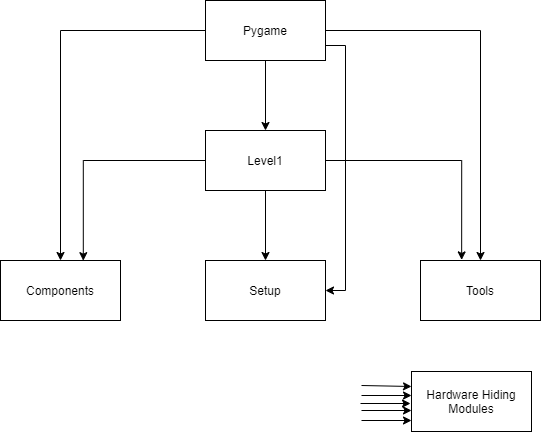
\includegraphics[width=0.7\textwidth]{UsesHierarchy.png}
\caption{Use hierarchy among modules}
\label{FigUH}
\end{figure}

%\section*{References}

\bibliographystyle {plainnat}
\bibliography {MG}

\end{document}